\noindent We define a \textit{tensor} as a multi-dimensional array of complex numbers, $A \in \mathbb{C}^{D_1 \times \ldots \times D_r}$, where $r$ is called the \textit{rank} of the tensor. Graphically, we represent a tensor as a geometric shape with one \textit{leg} attached for each index $\alpha_1, \ldots, \alpha_r$. There are three fundamental tensor operations:
\begin{itemize}
	\item \textit{Transposition}: Permuting the indices.
	
	\item \textit{Reshaping}: Merging or splitting legs. In particular, \textit{matricization} means dividing the legs into two groups, \textit{vectorization} means combining all legs into a single one. In analogy to the braket notation for physical states, we denote vectorized tensors by $\tket{A}$. The corresponding $\tbra{A}$ denotes its transpose, but without implicit complex conjugation: $\tbra{A} = \tket{A}^T$. This aligns with how tensors are stored and manipulated computationally.
	
	\item \textit{Contraction}: Connecting equal-dimensional legs of two tensors by summing over the corresponding indices and multiplying the tensor elements:
\begin{equation}\label{eq:contraction}
	\raisebox{-0.5\height}{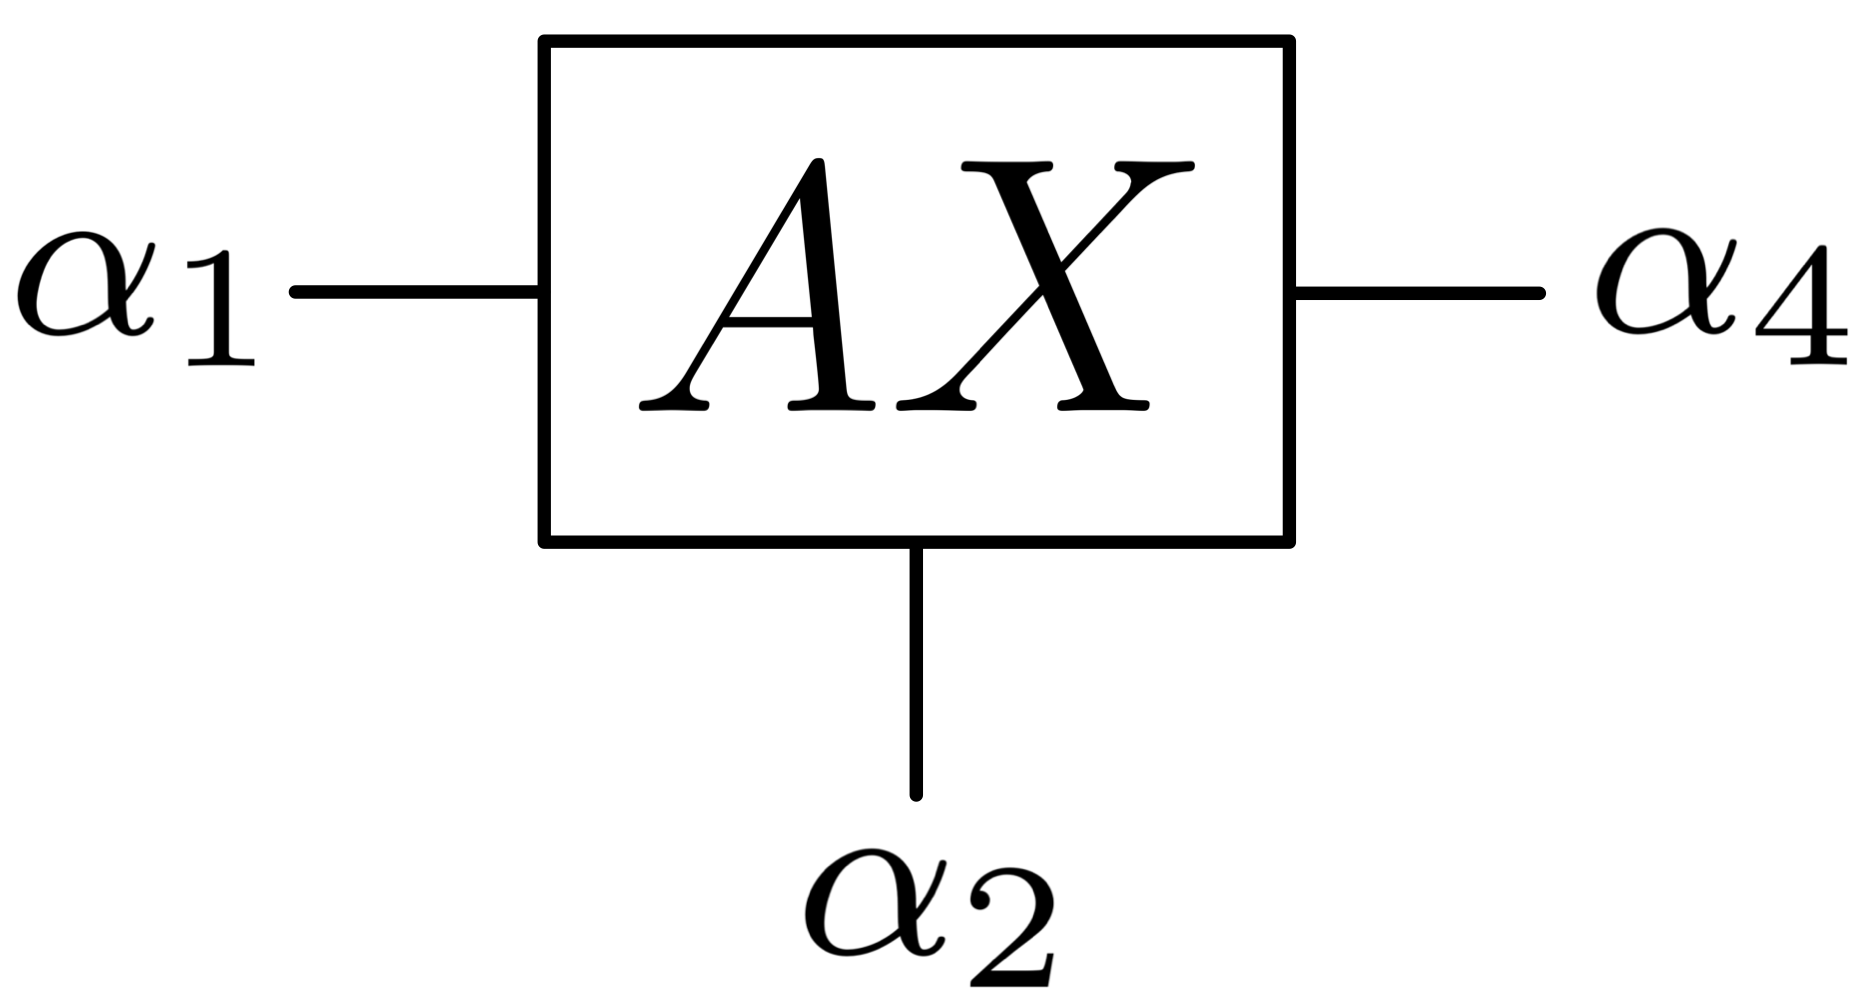
\includegraphics[height=1.2cm]{AX.png}}
	\: = \:
	 \raisebox{-0.5\height}{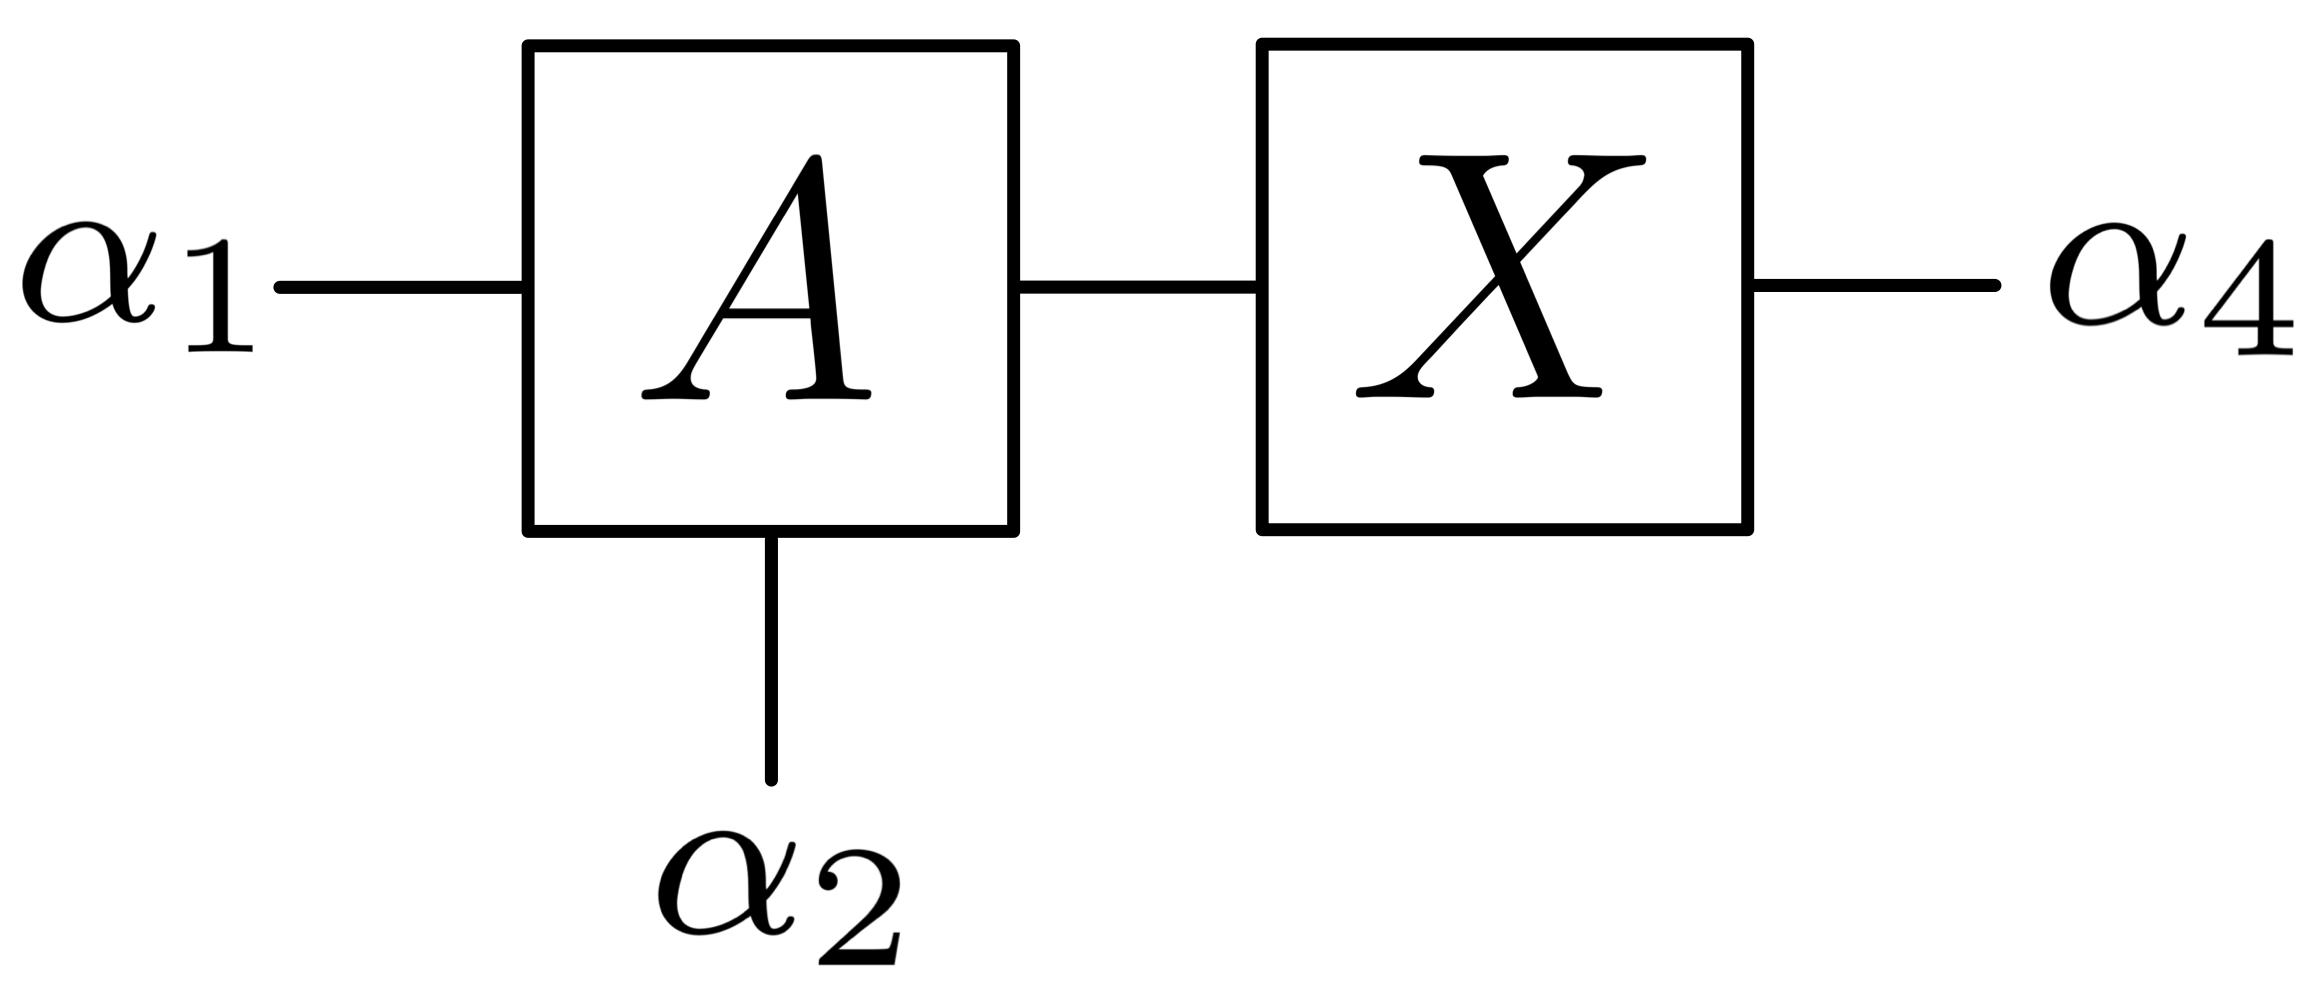
\includegraphics[height=1.3cm]{contraction.png}}
	 \: = \:
	\sum_{\alpha_3} A_{\alpha_1, \alpha_2, \alpha_3} X_{\alpha_3, \alpha_4} \:.
\end{equation}
The \textit{computational time complexity} is $\mathcal{O}[\text{dim(contracted legs)} \times \text{dim(open legs)}]$. A \textit{tensor network} is an arrangement of multiple tensors contracted with each other. The total contraction complexity can heavily depend on the pairwise contraction order. We draw a single outer shape for a tensor resulting from contractions described in its inside via diagrams or equations. The latter can be implicit about the legs being contracted, such as $AX$ in \eqref{eq:contraction}.
\end{itemize}

\noindent For two tensors of equal \textit{shape} $(D_1, \ldots, D_r)$, we define the general \textit{tensor inner product} as
\begin{equation}
	(A, B)_2  = \sum_{\alpha_1, \ldots, \alpha_r} \overline{A}_{\alpha_1, \ldots, \alpha_r} \: B_{\alpha_1, \ldots, \alpha_r}, 
\end{equation}
where the overline denotes complex conjugation. This coincides with the \textit{Hermitian inner product} $(\overline{A} \vert B)$ for vectors and the \textit{Frobenius inner product} $\text{tr}[A^{\dagger}B]$ for matrices. The induced norm is given by
\begin{equation}
	\Vert A \Vert_2 = \sqrt{(A, A)_2} = \left( \sum_{\alpha_1, \ldots, \alpha_r} \vert A_{\alpha_1, \ldots, \alpha_r} \vert^2 \right)^{1/2}.
\end{equation}

\noindent We call a tensor \textit{left/right isometric} if it can be reshaped into a matrix $A_L$/$A_R$ with orthonormal columns/rows, i.e. if $A_L^{\dagger}A_L = \mathbbm{1}$/$A_RA_R^{\dagger} = \mathbbm{1}$. We introduce ingoing and outgoing arrows on the legs such that the contraction of an isometric tensor with its complex conjugate over all ingoing legs yields the identity over all outgoing legs. The total Hilbert space dimension of the ingoing legs must be greater than or equal to that of the outgoing legs to permit an isometric map. For example, for $A_L, A_R \in \mathbb{C}^{D \times d \times D}$:
\begin{equation}
  \raisebox{-0.5\height}{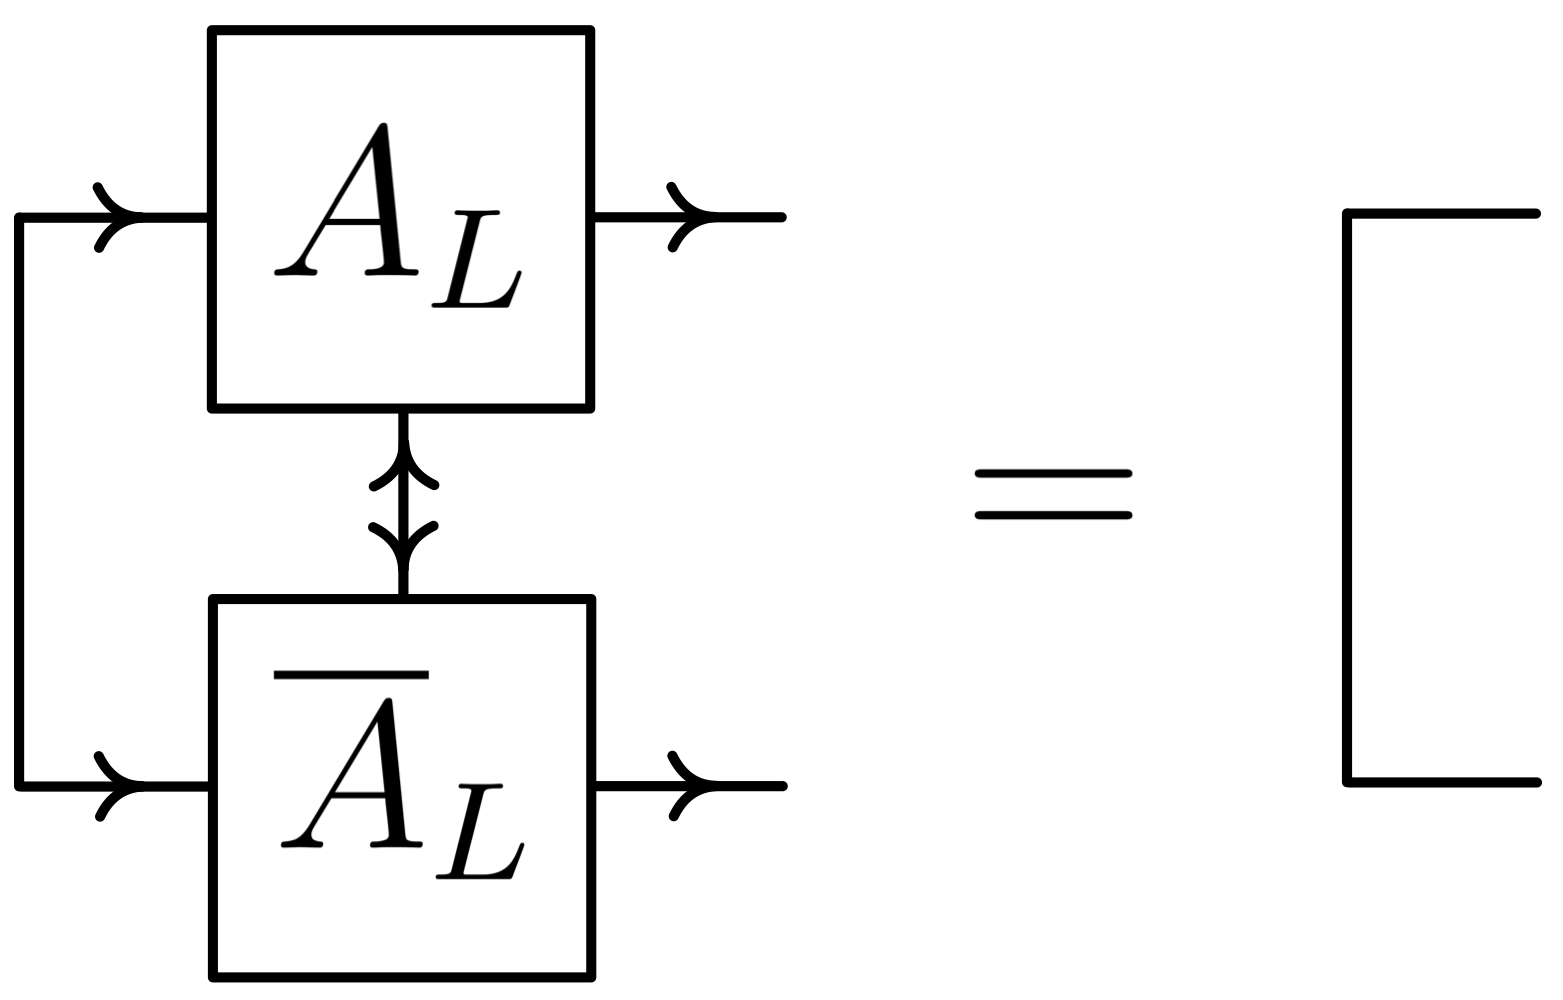
\includegraphics[height=2.1cm]{left_orthonormal.png}} \hspace{0.2em},
  \hspace{1em}
  \raisebox{-0.5\height}{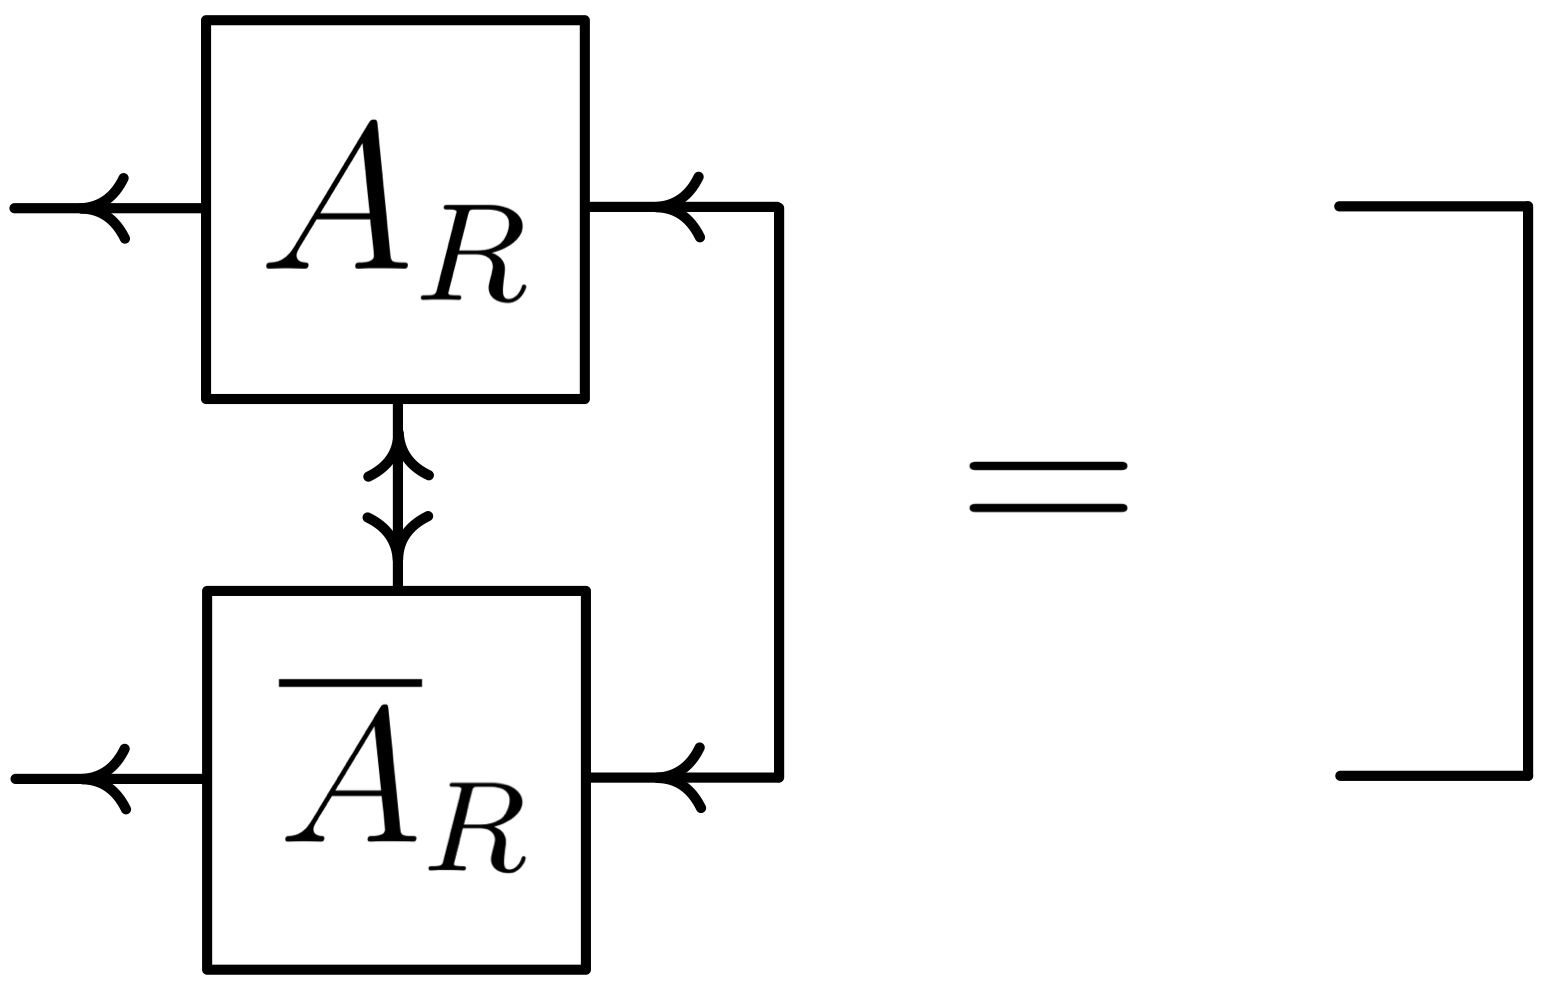
\includegraphics[height=2.1cm]{right_orthonormal.png}} \hspace{0.2em} .
\end{equation}

\vspace*{2em}

\noindent Any matrix $A \in \mathbb{C}^{M \times N}$ with $K = \min(M, N)$ admits the following standard decompositions involving isometric factors \cite{horn2012matrix}: \\

\noindent \makebox[\textwidth][s]{\parbox[b]{0.6\textwidth}{\underline{QR decomposition} $A = QR$} \hfill \raisebox{-0.3\height}{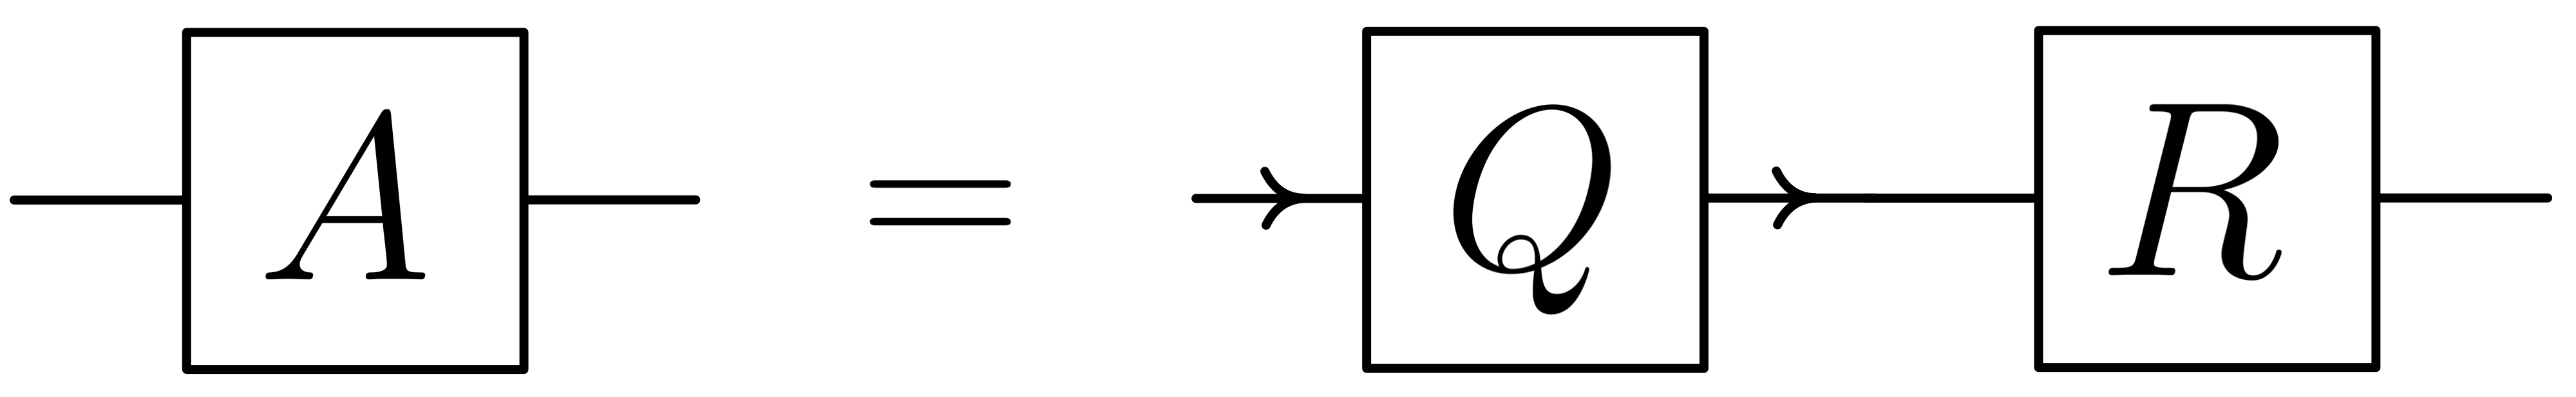
\includegraphics[height=0.8cm]{qr.png}}} \vspace{-0.75em} 
\begin{align}
\begin{split}
	& Q \in \mathbb{C}^{M \times K} \text{ left isometric } (Q^{\dagger}Q = \mathbbm{1}) \\
	& R \in \mathbb{C}^{K \times N} \text{ upper triangular } (R_{k,n} = 0 \text{ for } k > n) 
\end{split}
\end{align}
The computational runtime complexity scales as $\mathcal{O}(MKN)$. If $A$ has full rank, the decomposition can be made unique by ensuring that all main diagonal entries of $R$ are positive. Applying the QR decomposition to $A^T$ and transposing back goes under the name \textit{LQ decomposition}: $A = LQ$ with $L \in \mathbb{C}^{M \times K}$ lower triangular ($L_{m,k} = 0$ for $k > m$) and $Q \in \mathbb{C}^{K \times N}$ right isometric ($QQ^{\dagger} = \mathbbm{1}$). \\

\noindent \makebox[\textwidth][s]{\parbox[b]{0.6\textwidth}{\underline{Singular value decomposition (SVD)} $A = USV$} \hfill \raisebox{-0.3\height}{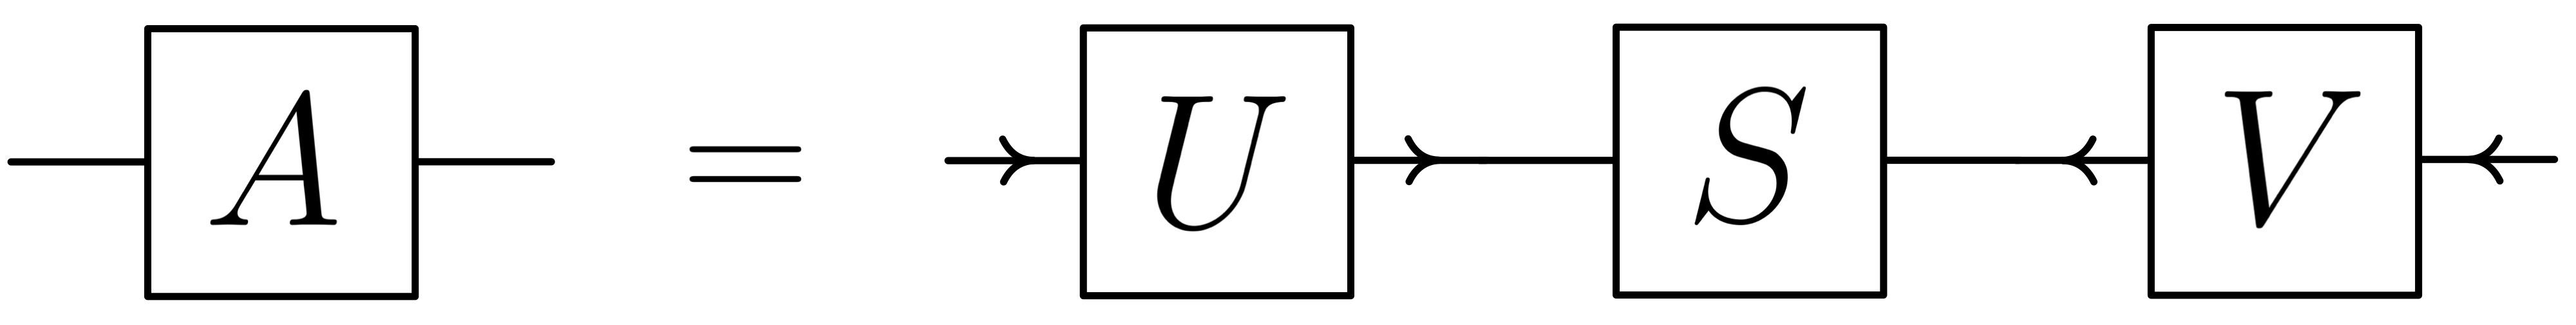
\includegraphics[height=0.8cm]{svd.png}}} \vspace{-0.75em} 
\begin{align}
\begin{split}
	& U \in \mathbb{C}^{M \times K} \text{ left isometric } (U^{\dagger}U = \mathbbm{1}) \\
	& S \in \mathbb{R}^{K \times K} \text{ diagonal, positive semidefinite, nonincreasing }  (S_{k,k} \equiv S_k \geq S_{k+1} \geq 0) \\
	& V \in \mathbb{C}^{K \times N} \text{ right isometric } (VV^{\dagger} = \mathbbm{1}) \\
\end{split}
\end{align}
The rank of $A$ is equal to the number of nonzero \textit{singular values} $S_k > 0$. Let us assume that this is $K$. We can define a \textit{truncation} of $A$ by keeping only the largest $D < K$ singular values:
\begin{equation}
	\Tilde{A} = \Tilde{U}\Tilde{S}\Tilde{V} \text{ with } \Tilde{U} = U_{[:, :D]}, \Tilde{S} = S_{[:D, :D]}, \Tilde{V} = V_{[:D, :]}.
\end{equation}
It can be proven that this is the best rank-$D$ approximation to $A$, with minimal \textit{truncation error}
\begin{equation}
	\varepsilon_{\text{trunc}} = \Vert \Tilde{A} - A \Vert_2 = \left( \sum_{k > D} S_k^2 \right)^{1/2}.
\end{equation}
As the QR decomposition (but with a larger prefactor), the computational runtime complexity scales as $\mathcal{O}(MKN)$. \\

\noindent \makebox[\textwidth][s]{\parbox[b]{0.4\textwidth}{\underline{Polar decomposition} $A = UP$} \hfill \raisebox{-0.3\height}{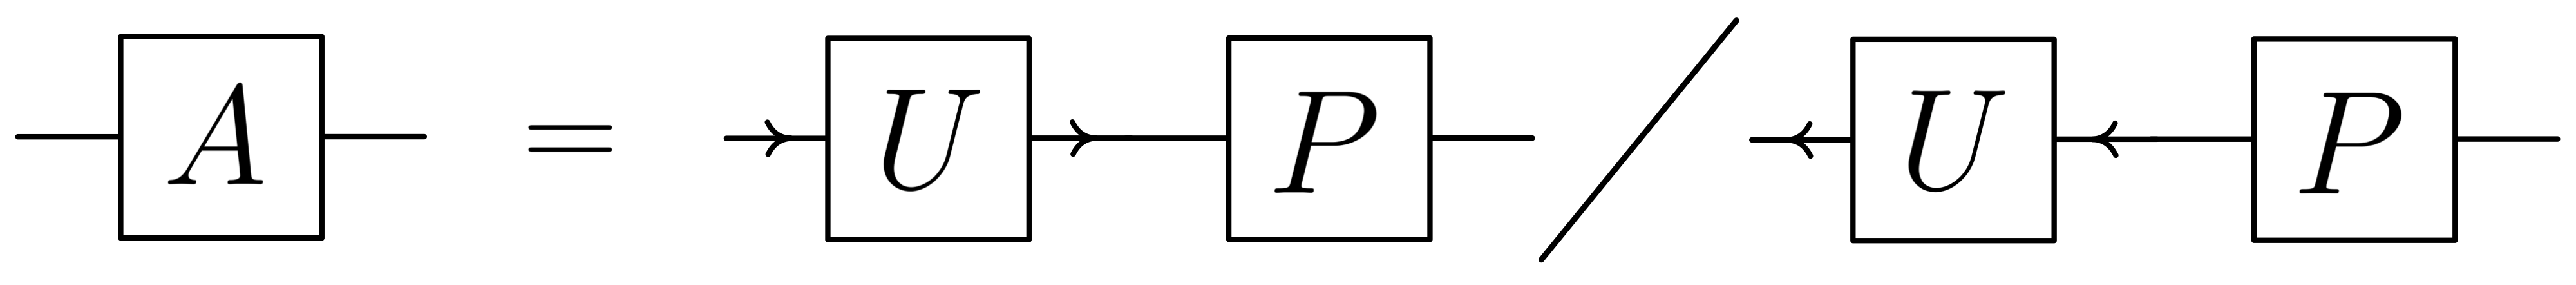
\includegraphics[height=0.9cm]{polar.png}}} \vspace{-0.75em} 
\begin{align}
\begin{split}
	& U \in \mathbb{C}^{M \times N} \text{ left isometric } (U^{\dagger}U = \mathbbm{1}) \text{ if } M \geq N, \text{ right isometric } (UU^{\dagger} = \mathbbm{1}) \text{ if } M \leq N \\
	& P \in \mathbb{C}^{N \times N} \text{ positive semidefinite }
\end{split}
\end{align}
We refer to this as the \textit{right polar decomposition}. A \textit{left polar decomposition} is obtained by applying a right polar decomposition to $A^T$ and transposing back: $A = PU$, where $P \in \mathbb{C}^{M \times M}$ is positive semidefinite, and $U$ again satisfies isometric conditions depending on the relative dimensions. Note that the polar decompositions can be easily derived from the singular value decomposition: Given $A = \Tilde{U} \Tilde{S} \Tilde{V}$, we insert an identity $\Tilde{V} \Tilde{V}^{\dagger}$ or $\Tilde{U}^{\dagger} \Tilde{U}$ to get 
\begin{equation}
	A = \underbrace{(\Tilde{U} \Tilde{V})}_{U} \underbrace{(\Tilde{V}^{\dagger} \Tilde{S} \Tilde{V})}_{P} 
	\text{ or } 
	A = \underbrace{(\Tilde{U} \Tilde{S} \Tilde{U}^{\dagger})}_{P} \underbrace{(\Tilde{U} \Tilde{V})}_{U}.
\end{equation}

\vspace*{2em}

\noindent \underline{Variational tensor network states} \\[0.5em]
\noindent A \textit{tensor network state} is a (high dimensional) quantum many body vector $\ket{\psi} \in \mathcal{H}$ decomposed into a network of (lower dimensional) tensors. For approximating ground states and lowest-lying excited states of a Hamiltonian $H$ with tensor network states, we deal with minimization problems of the form 
\begin{equation} \label{eq:optimization}
	\argmin_{X} \frac{\bra{\psi(\overline{X})} H \ket{\psi(X)}}{\langle \psi(\overline{X}) \vert \psi(X) \rangle},
\end{equation}
where we optimize over one single tensor $X$ of the network (while keeping all the others fixed). To enforce normalization of $\ket{\psi(X)}$, we introduce a Lagrange multiplier $\lambda$ and minimize the energy functional 
\begin{equation} \label{eq:energy_functional}
	F(X, \overline{X}, \lambda) = \bra{\psi(\overline{X})} H \ket{\psi(X)} - \lambda \left[ \langle \psi(\overline{X}) \vert \psi(X) \rangle - 1 \right].
\end{equation}
Taking the derivative with respect to all components of $\overline{X}$, we obtain the stationary condition
\begin{equation} \label{eq:stationary_condition}
	\partial_{\overline{X}} \bra{\psi(\overline{X})} H \ket{\psi(X)} - \lambda \partial_{\overline{X}} \langle \psi(\overline{X}) \vert \psi(X) \rangle = 0.
\end{equation}
We now introduce the \textit{effective Hamiltonian matrix}
\begin{equation}
	H_{\mathrm{eff}} = \partial_{X} \partial_{\overline{X}} \bra{\psi(\overline{X})} H \ket{\psi(X)},
\end{equation}
and the \textit{norm matrix}
\begin{equation} \label{eq:norm_matrix}
	N = \partial_{X}\partial_{\overline{X}}  \langle \psi(\overline{X}) \vert \psi(X) \rangle,
\end{equation}
whose networks are obtained by removing the tensors $X$, $\overline{X}$ from the networks $\bra{\psi(\overline{X})} H \ket{\psi(X)}$ and $ \langle \psi(\overline{X}) \vert \psi(X) \rangle$. The optimal tensor $X$ (rearranged as a vector) corresponds to the ground state of the generalized eigenvalue problem
\begin{equation} \label{eq:effective_eigenvalue_equation}
	H_{\mathrm{eff}} \tket{X} = \lambda N \tket{X}.
\end{equation}
Making sure that $X$ is completely surrounded by isometric tensors in $\ket{\psi(X)}$, the power of \textit{isometric tensor network states} is twofold. First, the norm matrix is just the identity matrix, so that the generalized eigenvalue problem reduces to a standard one. Second, local SVD truncations of $X$ become globally optimal. \\

\noindent In practice, there is usually no need for building the matrix $H_{\mathrm{eff}}$. Instead, one should only implement the matrix-vector multiplication $H_{\mathrm{eff}} \tket{X}$, by finding an optimal contraction path for the action of $H_{\mathrm{eff}}$ on $X$ on the tensor level. The ground state can then be efficiently computed using an iterative Lanczos method. \cite{orus2014practical}